\chapter{Musicality of the solutions}
This last chapter is concerned with the musicality of the solutions. Its objective is not anymore to discuss the best way to translate Fux's preference into costs, but to play a little bit with the possibilities offered by the tool. We try to change the costs in order to leave Fux's initial preferences and to see what it can yield as a result.

\section{Looking at the results of single species compositions}

\section{Trying custom costs}
Below is an example of the difference between a counterpoint of the first species, using Fux's preferences (more precisely, using a lexicographic search with default preferences as defined in Section \ref{section:lexicographic-order}), and a counterpoint in which personal preferences were expressed. These preferences were: to use as few contrary motions as possible, and as many oblique and direct motions as possible. Prioritising this preference (placing it first in the lexicographic order), then prioritising melodic intervals (maintaining a preference for small melodic intervals, as in \gap), then prioritising variety, and then placing all the other preferences at the penultimate level of the lexicographic order, with the exception of the preference for no successive perfect consonance, which was placed at the very last level.

The search has not been stopped manually; we leave it running until it finds the best solution according to the defined preferences.

The aim of this experiment is twofold: to show that changing the order of the preferences has an effect on the solution, which was already partially demonstrated in the previous chapter, and to obtain a much more monotonous solution than the Fux-like solutions (for example, for transitions between two parts of a composition, for more quiet moments, ...).

The results of this experiment can be found in figures \ref{fig:musicality-1sp-fux} and \ref{fig:musicality-1sp-custom}.
\begin{figure}[h]
    \centering
    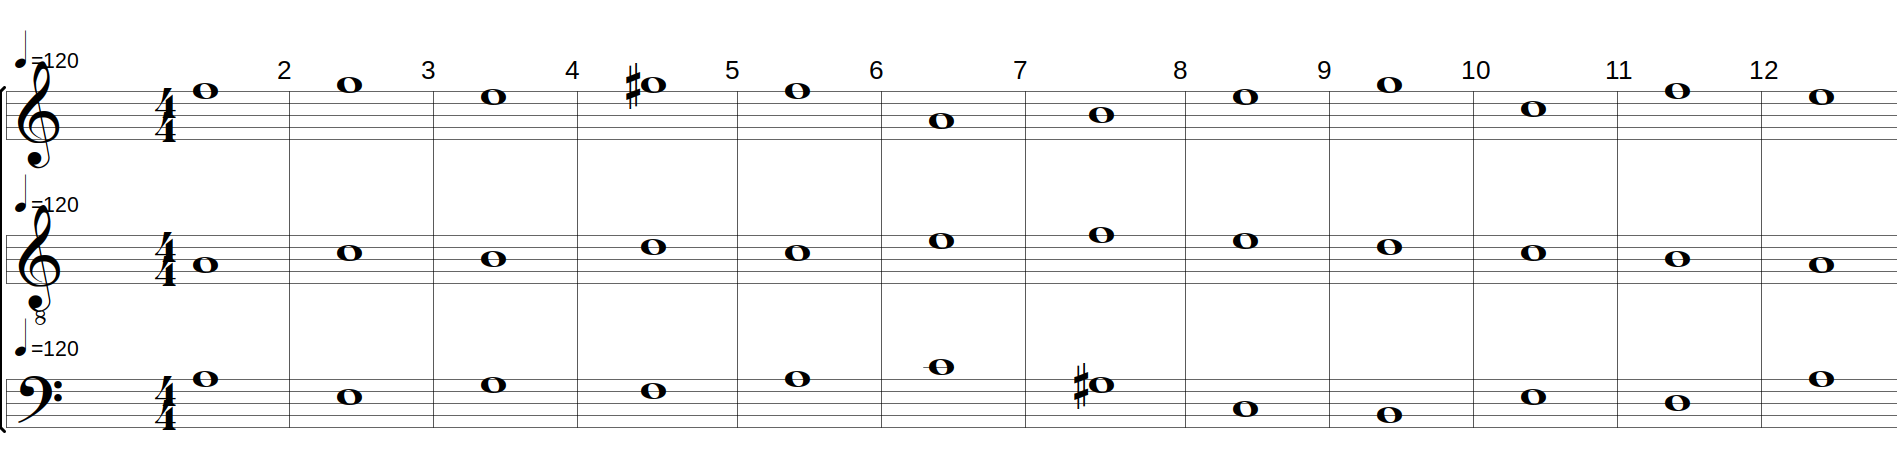
\includegraphics[width=1\textwidth]{Images/Musicality/musicality-1sp-fux-pref.png}
    \caption{Example of a first species counterpoint in three-part composition with Fux's preferences}
    \label{fig:musicality-1sp-fux}
\end{figure}

\begin{figure}[h]
    \centering
    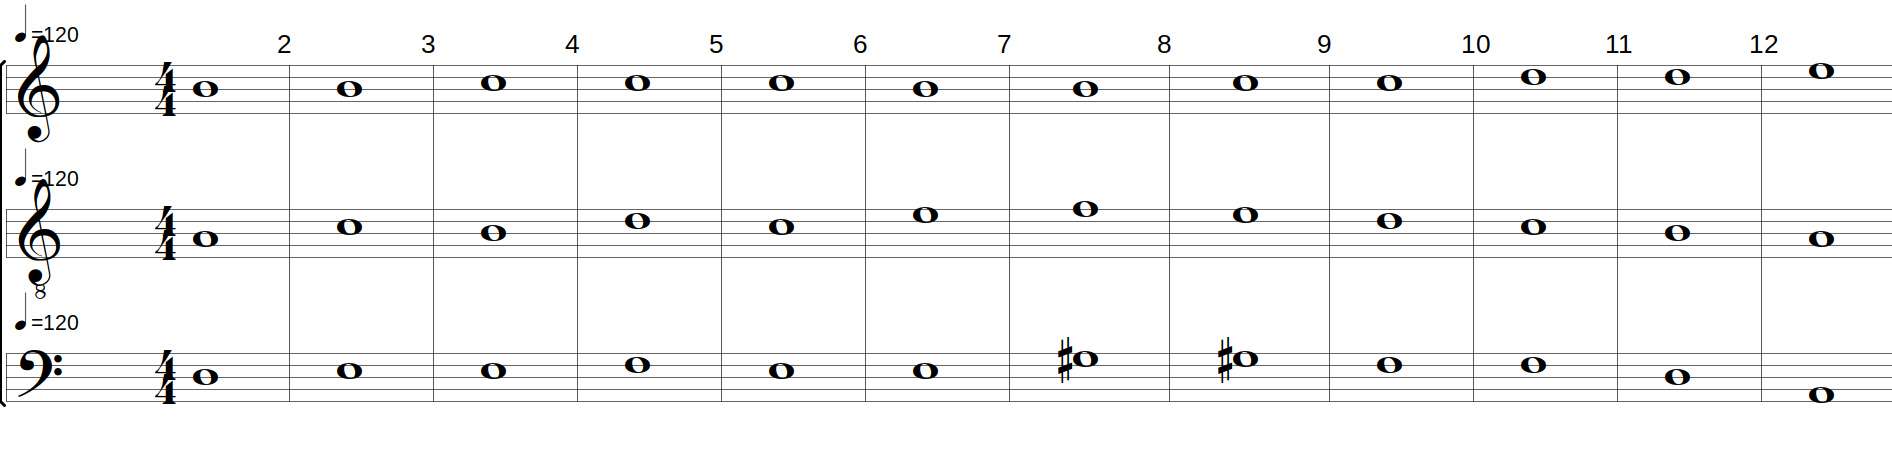
\includegraphics[width=1\textwidth]{Images/Musicality/musicality-1sp-custom-pref.png}
    \caption{Example of a first species counterpoint in three-part composition with custom preferences}
    \label{fig:musicality-1sp-custom}
\end{figure}

The result is striking, as the Fux-like solution simply sounds like... Fux, and the custom solution is completely in line with its aim, which was to create a composition that is more monotonous and where there is less sense of things happening.

\section{Analysing the results of mixing species}
If there's one thing that's clear about multi-species composition, it's that it's a truly unpredictable art. It has already been discussed in the \ref{section:time-to-find-a-solution} section that the different interactions between species, voice ranges and \textit{cantus firmi} can take more or less time in terms of solver efficiency. This is also true for the quality of the solutions, and there are times when the solver gives completely correct results, and times when the solution leaves a lot to be desired. This lack of musical quality in the solutions was not the case when we were composing single species counterpoints (without mixing the species), and is something that emerges when combining species. The most plausible hypothesis is that the solver is unable to produce a solution that is \textit{always} beautiful when combining species precisely because Fux has never given any rules specifying how to combine species. We can only hope that such rules exist in the 3rd chapter of his book, or else we'll have to either extrapolate from existing rules or take inspiration from other authors to create these rules.

Below (Figures \ref{fig:musicality-5sp-la} and \ref{fig:musicality-5sp-do}) are two examples of counterpoint generated by FuxCP. Both combine counterpoint of the second kind and counterpoint of the fifth species. The search ran for three minutes before being interrupted.

\begin{figure}[h]
    \centering
    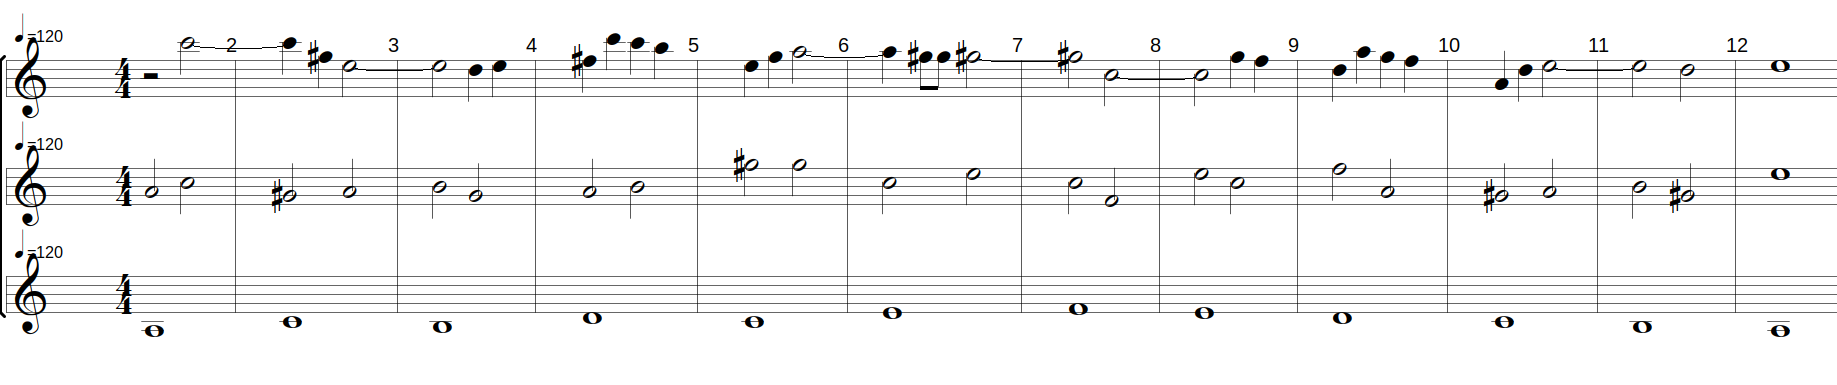
\includegraphics[width=1\textwidth]{Images/Musicality/musicality-5sp-la.png}
    \caption{Example of a generated counterpoint using a second species counterpoint and a fifth species counterpoint, with in an A scale.}
    \label{fig:musicality-5sp-la}
\end{figure}

\begin{figure}[h]
    \centering
    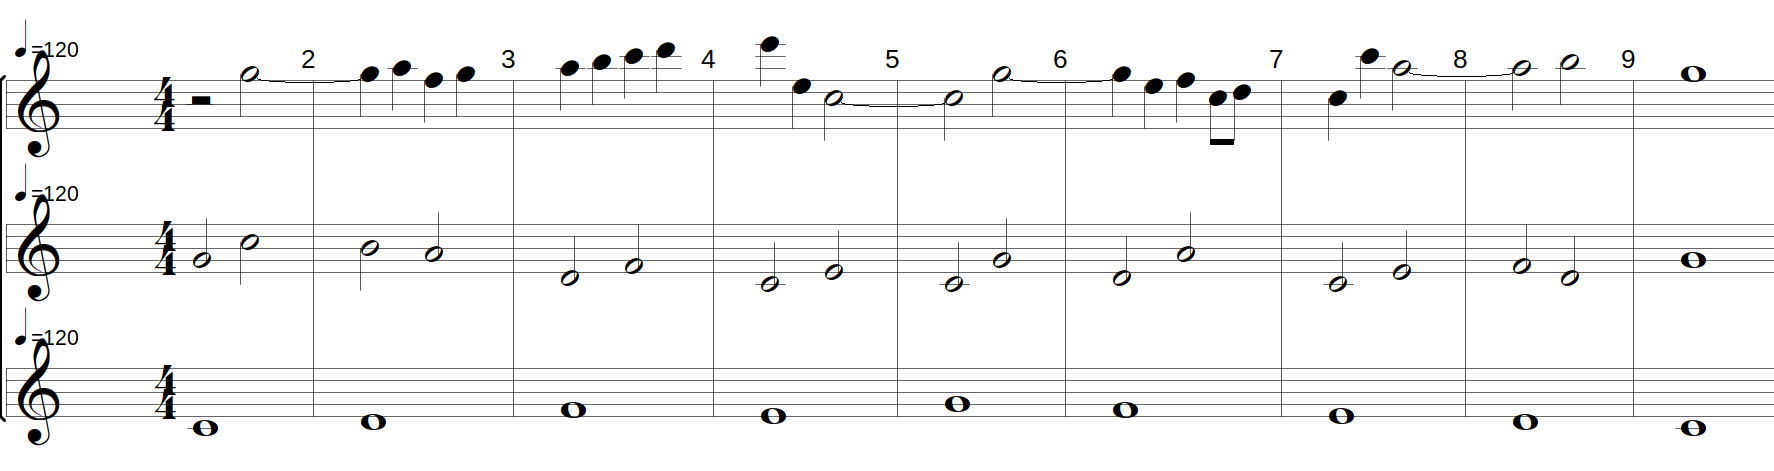
\includegraphics[width=1\textwidth]{Images/Musicality/musicality-5sp-do.png}
    \caption{Example of a generated counterpoint using a second species counterpoint and a fifth species counterpoint, with in a C scale.}
    \label{fig:musicality-5sp-do}
\end{figure}